\documentclass[conference]{IEEEtran}
\IEEEoverridecommandlockouts
% The preceding line is only needed to identify funding in the first footnote. If that is unneeded, please comment it out.
\usepackage{cite}
\usepackage{amsmath,amssymb,amsfonts}
\usepackage{algorithmic}
\usepackage{graphicx}
\usepackage{textcomp}
\usepackage{xcolor}
\usepackage{geometry}
\usepackage{float}
\usepackage{adjustbox}

\usepackage{biblatex} %Imports biblatex package
\addbibresource{references.bib}
\graphicspath{ {./Images/} }

\begin{document}
\title{
A Study Into The Applications of Machine Learning in The Diagnosis \& The Prognostication of Breast Cancer\\
\vspace{5mm}
\large Department of Computing \\
\vspace{3mm} 
\large Letterkenny Institute of Technology \\
\vspace{3mm} 
\large Machine Learning
}
\vspace{3mm}  
\author{Ultan Kearns \& Liam Millar}
\maketitle
\begin{abstract}
    Machine Learning has been used in a variety of healthcare fields and has proven to be very successful in regards to automating / helping with certain tasks ranging from identifying similarities in different strains of DNA and making inferences on new DNA strains to diagnosing various types of diseases and predicting the prognosis from sample data.  Machine Learning is particularly useful when it comes to analyzing and comparing data, this data can then be used to train a model to notice certain similarities in malignant and benign tumours.  This paper aims to analyze which methods would be best suited to identifying factors which contribute to a cancer being malignant or benign and to predict the prognosis of breast cancer based on those factors.\\
    keywords - Machine Learning, Breast Cancer, Prognosis, Diagnosis
\end{abstract}

\section{Introduction}
Machine Learning is a field which aims to train machines to think and learn like humans.  This is done by feeding data into the machine, the machine then analyzes the data and begins to start noticing patterns within the data and starts to create a model, this model can be used to train the machine so that when new data is feed in the machine can easily detect certain characteristics about the data and classify it.  Machine Learning is a subset of AI which is comprised of many fields, and has been proven to perform very well in predicting outcomes in a large variety of areas such as STEM fields, Economics, Social Sciences and various others.  The ultimate goal of machine learning is to train a machine to perform a task without any human intervention and to learn to adapt to new data and new patterns which appear in the data.  There has been an increased reliance on machine learning in the past few years and it has become ubiquitous in the modern world.\\

There are many ways which a machine may choose to learn we will explain the types of learning we used when trying this model in the upcoming sections.

\subsection{Supervised Learning}
Supervised learning is a type of machine learning that involves training a machine with labelled training data to make inferences about new data.  The machine reads in the data and begins to notice certain patterns from it and uses the learned patterns to make inferences about new data.  There are many algorithms which can be used in supervised learning, we will list a few we used below.  
\vspace{2mm}
\subsubsection{Linear Regression}
This algorithm involves finding a line to best fit the data, this is achieved by modifying parameters to find the best fitting line for a given dataset. This method works by learning to predict a pattern within the data and drawing a line through a series of data points so that the line fits is close to as many of the points as possible, in this way we can make predictions by seeing how closely a given point would fit our line.  
\vspace{2mm}
\subsubsection{Naive Bayes}
Naive Bayes is a technique which makes features of an object have the same weight when trying to classify the data.  This algorithm works well on small data sets and it can improve the results of a model when working with a limited dataset.  An example of Naive Bayes would be to train an image classifier for identifying cars, using Naive Bayes the property of a cars wheels would have just as much impact as the number of doors of the car.
\subsection{Unsupervised Learning}
Unsupervised learning is a type of machine learning where the machine is not provided with any labelled data and makes inferences about the data based on patterns found in the training data, the most common types of unsupervised learning are reinforcement learning which "rewards" a machine for performing in a certain way and "punishes" it for acting in the "wrong way" and clustering which groups data together based on similar features.
\subsubsection{Random Forest}
\subsubsection{K Nearest Neighbour}
K Nearest Neighbour is an algorithm which measures the distance between data points by using a distance metric eg: Cosine distance, Euclidean distance, Jaccardian distance etc and groups data points which are near each other into clusters.  In K Nearest Neighbour we make the assumption that data points within a certain distance must have some common properties or features, in this way we can separate the data into groups which share these features.

\subsection{Breast Cancer}
Breast cancer is a type of cancer which forms in the breast tissue, it has many signs and symptoms such as: 
\begin{itemize}
    \item New lump in the breast or underarm (armpit).
    \item Thickening or swelling of part of the breast.
    \item Irritation or dimpling of breast skin.
    \item Redness or flaky skin in the nipple area or the breast.
    \item Pulling in of the nipple or pain in the nipple area.
    \item Nipple discharge other than breast milk, including blood.
    \item Any change in the size or the shape of the breast.
    \item Pain in any area of the breast.
\end{itemize} \cite{symptomsofbreastcancer}
\\
\\
Breast cancer is also one of the most common occurring cancers in women and the average risk of a woman developing cancer in her lifetime is about 13\% or 1/8 in the United States alone\cite{howcommonisbreastcancer} and in 2020 there were 2.3 million women diagnosed with the disease of which 685,000 succumbed to the disease\cite{breastcancerstatistics}. In Ireland 3,700 new cases of breast cancer are diagnosed each year\cite{breastcancerireland}. Breast cancer treatment is has a very high survival rate if caught early, the survival rate for those in high income countries was 90\% \cite{breastcancerstatistics}.
\subsection{Discuss various uses of machine learning in medicine today}
\subsection{Libraries we used in this project}
I have listed the libraries we have used in this project below:
\begin{itemize}
    \item numpy referred to throughout our notebook as np\cite{numpy}  - the Numpy library was used to perform numerical operations on our dataset
    \item pandas referred to throughout our notebook as pd \cite{pandas} - Pandas was used to create dataframes from our dataset
    \item sklearn referred to throughout our notebook as sk \cite{sklearn} - We used SKlearn to implement many of our models and to output statistics relating to the models.
    \item matplotlib \cite{matplotlib} - We Used the matplotlib library to create visual interpretations of our data
    \item google.colab \cite{googlecolab} - Google Colab was used to upload our data set and also as an editor so we could compile and run our Jupyter Notebook\cite{jupyter}
\end{itemize}
\subsection{Aims of the project}
 The aim of this project is to train a model using machine learning to analyze data from both benign and malignant tumours to detect patterns in the data and to predict whether tumours will be malignant or benign given certain parameters with reasonable accuracy.
\section{Methodology}
\subsection{Creating testing and training sets}
We created testing and training sets from the data set by splitting the data set using the Sklearn Library\cite{sklearn} and creating four dataframes two for our X \& Y test sets and two more for our X \& Y training sets.  We then used the training sets to train a variety of models to make predictions about our test sets, we then measured the models performance based on how accurately it predicted data in the test set.  We used a variety of metrics to compare our data when using different models and gauged how accurately they performed on our test data.  When deciding how we should split the data we experimented with a number of values to decide on which split best suited our models, we determined this through trial and error rerunning our models with different splits to determine which split yielded the most accurate prediction.  
\subsection{Cleaning The Data}
The dataset we used was the Breast Cancer Wisconsin (Diagnostic) \cite{misc_breast_cancer_wisconsin_17}. This dataset consists of features computed from digitized images of fine needle aspirate (FNA) of breast mass. It contains 569 instances(rows) and 32 variables(cols). There are 2 categorical variables ID and Diagnosis(our target). There is also 30 continuous variables used to describe the features broken into 3 sets of ten measurements using different methods. There were no missing data in this set so no imputation methods needed to be used.
When starting the project we noticed that some of the data corresponded highly with other data, we then decided to remove these columns to increase the speed of the model.  I have included an image below to show a positive correlation between the Mean Radius and Mean Perimeter columns.  We also changed the diagnosis columns from 'M' for malignant and 'B' for benign to 1 for malignant and 0 for benign, this made the data much easier to work with and helped us in performing various algorithms with it.
\begin{figure}[H] 
\caption{Example of a positive linear correlation between the mean radius \& perimeter, if the lines slope was the inverse of our current line that would be an example of high negative correlation and we would not have needed to remove these columns from our data set}
\centering
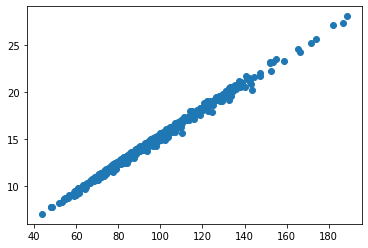
\includegraphics[height=50mm,width=0.5\textwidth]{positive_correlation.png}
\end{figure}
We were able to find this highly correlated data by using Pearson's correlation and I will include an image of the correlation in our dataset below
\begin{figure}[H]
\caption{Example of highly correlated variables in our data set as you can see the mean area corresponds highly with the data highlighted}
\centering
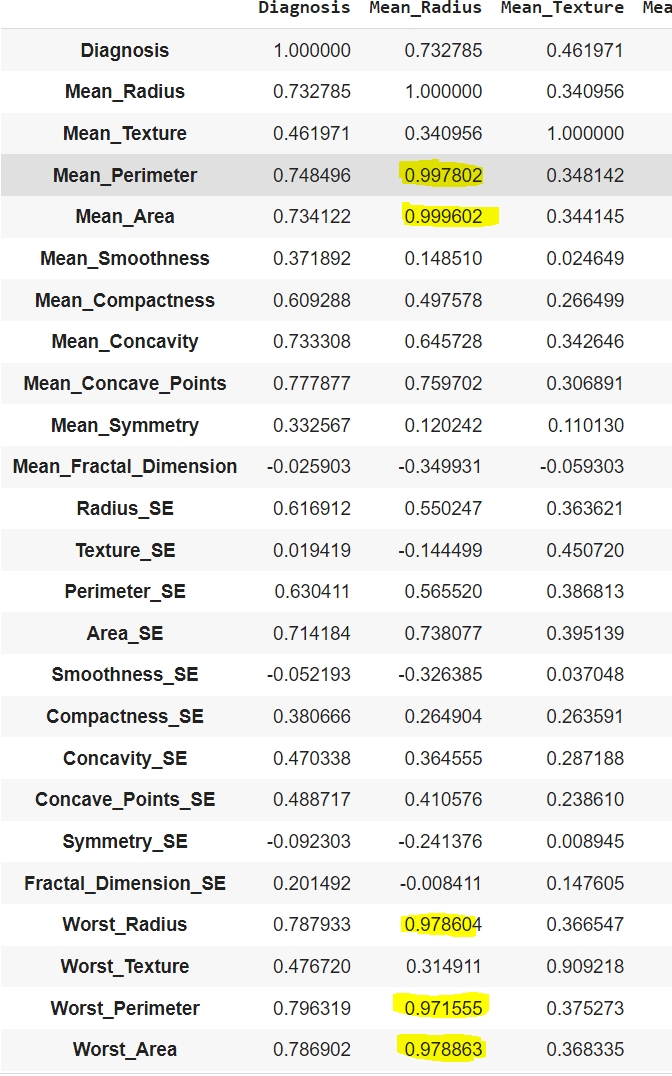
\includegraphics[height=80mm,width=0.5\textwidth]{dataset_correlation.PNG}
\end{figure}
Additionally we produced a heat-map of the correlations.
\begin{figure}[H]
\caption{The heat-map of correlations. This indicates a clear correlation between some of the columns and the complexity emphasises the need to reduce these columns where possible.}
\centering
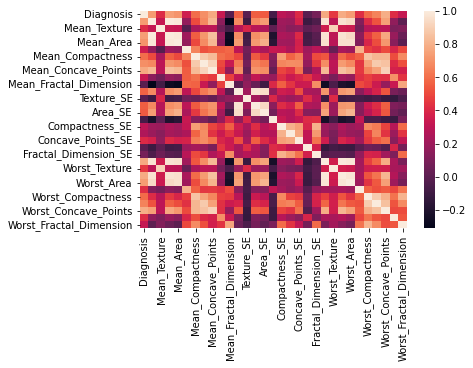
\includegraphics[height=60mm,width=0.5\textwidth]{correlation_heatmap.PNG}
\end{figure}
\subsection{Algorithms}
\subsubsection{Linear Regression}
In the notebook we used linear regression to predict values from our X and Y testsets based on features in our training sets.  We decided to use  Mean Radius  and Mean Fractal Dimension as an example of our negatively skewed linear regression model.  Our dependent variable was the Mean Radius and our independent variable was the Mean Fractal Dimension.   We trained the model by first creating our X training set and test set which contained the Mean Radius feature then we created our y training and testing set by using the Mean Fractal Dimension, we then reshaped the training and test data into a 2d array containing our feature values.  We then fit a model to display our results as we can see in the image below the relation between Smoothness Severity and Mean Radius is negatively correlated.
\begin{figure}[H]
\caption{Linear Regression Model of Mean Fractal and Mean Radius.}
\centering
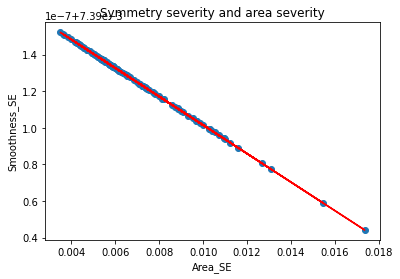
\includegraphics[height=60mm,width=0.5\textwidth]{Images/negatively_skewed_linear_regression.png}
\end{figure}
For our second linear regression model we decided to use two features which were highly correlated Concave Points Severity \& Concavity Severity our independent variable was the  Concavity Severity which we used to predict the dependent variable which was the Concave Points Severity.  As you can see from the image below the data was highly correlated and thus gave us the inverse line of the above negatively skewed model.
\begin{figure}[H]
\caption{Linear Regression Model of Concave Points Severity and Concavity Severity.}
\centering
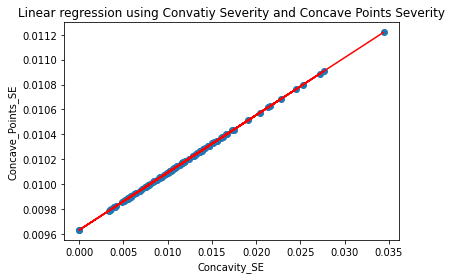
\includegraphics[height=60mm,width=0.5\textwidth]{Images/positively_skewed_linear_regression.png}
\end{figure}
\subsubsection{Decision Trees}
Decision Trees are a form of supervised learning that construct a flow chart from a set of training data and its results. This flow chart allows the prediction of future results based on a comparison to the features. However they can be prone to over fitting as all future decisions are based on the importance attributed to features of the training data. As part of or exploration of the data set we did a side by side comparison of decision trees based on information gain(entropy) and the gini index(gini) methods.
From our results we discovered that while both methods provided quite accurate results 0.9005847953216374 or about 90.0\% for information gain and 0.9298245614035088, or about 93.0\% for the gini method. the scikit default gini proved to be the most accurate.
\subsubsection{Random Forest} Random Forest is used to construct multiple decision trees from samples of the training data in order not to limit its scope and try to alleviate some of the issues with over fitting and precision that can occur with a single decision tree, this collection of trees produce separate predictions that are used as votes to form a majority decision on the final predicted result. We used the same data split to test using the random forests for both gini and entropy(information gain), once again accuracy was high with 0.9473684210526315 or 94.7\% for gini and 0.935672514619883 0r 93.6\% for entropy, these values varied a little for the random forest due to the randomness but they remain consistently higher than the respective decision tree model and even the entropy random tree models accuracy improved upon the gini singular decision tree. 
\subsubsection{Cross Validation} Because our dataset was reasonably small we ran some cross validation testing on the tree and random forest models 
\subsubsection{Naive Bayes}
We implemented Naive Bayes in our notebook by using the following features Radius Severity, Texture Severity, Perimeter Severity, Area Severity, Smoothness Severity, Compactness Severity, Concavity Severity, Concave Points Severity, Symmetry Severity, Fractal Dimension Severity to train a model to predict the diagnosis of breast cancer.  We choose the following features because they seemed to have a high impact on the diagnosis and some had a low correlation value with others which provided our model with a variety of features which were different from one another which allowed our model to predict more accurately.
\subsubsection{K Nearest Neighbour}
We implemented K Nearest Neighbour by creating a new training set with the diagnosis dropped and defining a test set based on the y test diagnosis values, the model was then trained using the new training set and the diagnosis values with the y training set.  We chose a value of 25 for the neighbours we've passed in to the model as this yielded the best results.  We then tested the model by comparing values in our test array to the predicted values of our model, the model was right 26 out of 30 times, giving it an ~86\% accuracy rating.
\subsection{Machine Learning Techniques}
\section{Challenges}
\subsection{Over fitting}
Over fitting occurs when the model is performing very well on the training data but performs poorly on new data, this is due to the fact that the model has been trained to fit the training data so well that it cannot adapt to different data. To try and alleviate this we performed dimensionality reduction to find the features that are discriminative.
\subsubsection{Principal Component Analysis(PCA)} This is a form of unsupervised dimensionality-reduction and as our dataset contained a high number of features 30 we also explored the possibility of reducing these features by finding principle components that retain the essential parts of the data with the most variation while eliminating the sections that had little variation and less essential. A number of the features we saw were highly correlative as they were  derived from each other such as radius, diameter and area of a circle. This implied that PCA was a good method of dimensionality reduction to explore. We standardised the dataset to remove the impact of diverse measurement scales.
\subsection{Under fitting}
When training the models we also had to worry about underfitting the data, underfitting occurs when the model does not predict well enough on either the training or test sets.  Such a model is not practical and has no purpose or uses.
\section{Applications}
\subsection{Diagnosis of Breast Cancer}
The KNN model has a fairly accurate prediction of the diagnosis as does our first Naive Bayes model, as with all diagnostics tools there will need to be a doctor on hand also to analyze the information in case the AI generates false negatives or false positives.  The models do provide however an insight into whether a tumour is benign or malignant.
\subsection{Prognosis of Breast Cancer}
The models can predict whether a tumour will be malignant or benign from features in our dataset this means that doctors can feed in the values of said features and produce a prognosis indicating the possibility of the tumour being benign or malignant.
\section{Conclusion}
\subsection{Accuracy of Models}
\subsubsection{Naive Bayes}
We defined two Naive Bayes models for our paper the first predicted very accurately and was given more features we achieved perfect scores with all of our testsets which indicated the model was possibly overfitted.  We then decided to make a second model with less features this model suffered greatly generally only predicting one value for all training / testsets this is due to underfitting the model.
\subsubsection{KNN}
The KNN model predicts fairly accurately when the training / test split is 0.5, below I will include the correctly predicted values out of the actual values.
\\
X\_test: Total values:  285  correctly predicted values:  259 or 90\%
\\
X\_train:  Total values:  284  correctly predicted values:  272 or 95\%
\\
y\_test: Total values:  285  correctly predicted values:  263 or 92\%
\\
y\_train: Total values:  284  correctly predicted values:  273 or 96\%
\\
From the above results we can see that this technique works very well with our dataset with around 9 / 10 predictions being accurate. 
\subsection{What could be done differently}
Our dataset was quite small which would lead to some concerns about over fitting for the training data especially for the likes of decision tree. We took steps to alleviate some of the concerns about this. For the purpose of our exercise this was fine but ideally an expanded set of real world data points for training would ensure a more confident outcome.
\newpage
\clearpage
\tableofcontents
\printbibliography
\listoffigures
\end{document}
